% !TEX root = ../thesis.tex
\chapter{Background}
This chapter will go over definitions and background knowledge
necessary for understanding the methodology and evaluation presented in later chapters.
It will adress fundamentals of Business Process Management, go over the basics of neural networks and decision trees,
and explain how fairness is quantified in this thesis.

\section{Business Process Management}
\textbf{Business processes} represent structured sets of activities
or tasks undertaken by organizations to achieve specific objectives,
such as processing customer orders, managing inventory or onboarding new employees.
A specific execution or instance of the overall business process is refered to as a \textbf{case}.
For example, in an order fulfillment process, each order corresponds to a separate case.

\subsection{Business Process Model and Notation}
In order to provide visualization for stakeholders,
business processes are often portrayed in the form of \textbf{process models}.
These capture the sequence and flow in a formalized representation
and are generally created using the standardized
\textbf{Business Process Model and Notation (BPMN)} \cite{bpmn},
which we will also use a simplified subset of:

\begin{itemize}
\item \textbf{Activities} are represented as rectangles with rounded corners,
denoting the individual tasks or operations within the process.
\item \textbf{Gateways} are represented as diamond shapes with a cross inside and are used to manage the branching and merging of process flows.
They serve as decision points where the workflow can split into different paths or converge back into a single path.
In this thesis, we focus only on exclusive decision points, meaning that only one of the available paths can be taken at any given time.
The probability of choosing each path will be explicitly annotated.
\item \textbf{Events} are shown as circles,
representing the initiation and completion of the process.
Specifically, the start event,
depicted as a circle with a narrow border, marks the beginning of the process
and the end event, depicted as a circle with a bold border, signifies the process's conclusion.
\item \textbf{Sequence Flow} is represented by lines with solid arrowheads
and is used to show the order that activities will be performed in.
\end{itemize}

\begin{figure}[h!]
    \centering
    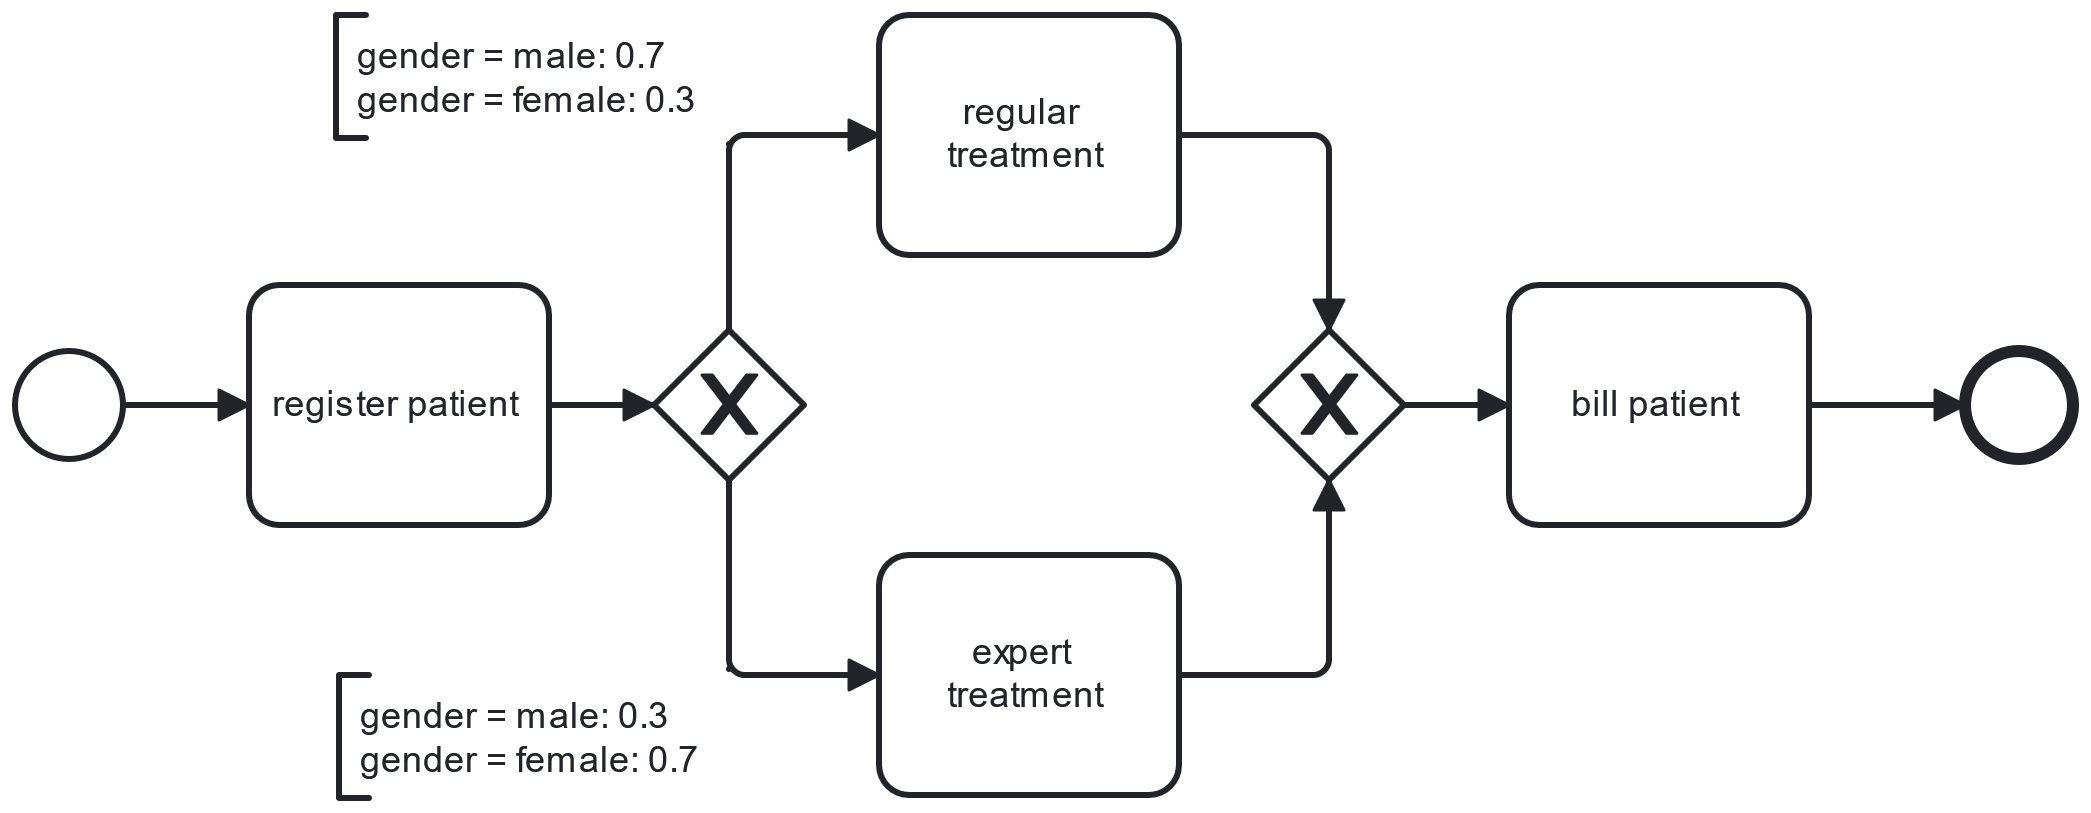
\includegraphics[width=\textwidth]{gfx/showcase.png}
    \caption{A simplified process model in BPMN describing the treatment of patients in a hospital.
    The branches of the gateway are annotated with transition probabilities based on the case attribute \textit{gender}.}
    \label{fig:bpmn_example}
\end{figure}

\subsection{Event Log Data}
\label{sec:event_log}
During the execution of business processes, data is captured and stored in the form of event logs.
To formally define the structure of this data,
let $A$ be the universe of all process activities,
$C$ the universe of case IDs,
$T$ the universe of possible timestamps
and $S_1, ..., S_m$ the universes of the $m$ attributes associated with the process.

In this thesis, we focus exclusively on \textbf{case attributes},
which are static and remain unchanged throughout the execution of a process instance.
These attributes describe characteristics of the process instance itself,
rather than dynamic properties of individual events.
Case attributes can be either \textbf{categorical},
containing predefined categories or classes, such as the patients gender or nationality,
or \textbf{numerical}, representing continuous or discrete numerical values, like the patient's age or income. 

In an event log, executed activities are recorded as individual events.
Each \textbf{event} $e$ can be formally described as a tuple $e = (a, c, s, t)$.
Here, $a \in A$ is the activity that has been executed,
$c \in C$ is the case ID, linking the event to a specific process instance,
$s$ is a tuple $s = (s_1, ..., s_m)$ with $s_i \in S_i, \forall i \in \{1, ..., m\}$,
containing the values of each attribute
and $t \in T$ is the timestamp denoting when the event occurred.

The sequence of all events $e_1, ..., e_l$ belonging to a single case $c$,
ordered by their timestamps, is called the \textbf{trace} of $c$ with length $l$.
Considering that a trace describes the life-cycle of a single case $c$,
all events belonging to a trace have the same attribute values $s$.
A \textbf{prefix} with length $l'$ is a portion of such a trace with length $l$,
consisting of the first $l'$ events, with $l' < l$.
Finally, an \textbf{event log} is a finite collection of traces belonging to the same process.

\begin{table}[h!]
    \centering
    \scriptsize
    \renewcommand{\arraystretch}{1.2}
    \setlength{\tabcolsep}{6pt}
    \begin{tabular}{>{\centering\arraybackslash}m{1.2cm} | m{3cm} | m{3.5cm} | m{1.5cm}}
        \toprule
        \textbf{Case ID} & \textbf{Activity} & \textbf{Timestamp} & \textbf{Gender} \\
        \midrule
        1 & Register Patient & 2025-02-08 09:15:00 & Male \\
        1 & Expert Treatment & 2025-02-08 09:30:00 & Male \\
        1 & Bill Patient & 2025-02-08 09:45:00 & Male \\
        \midrule
        2 & Register Patient & 2025-02-08 10:05:00 & Female \\
        2 & Regular Treatment & 2025-02-08 10:20:00 & Female \\
        2 & Bill Patient & 2025-02-08 10:35:00 & Female \\
        \midrule
        3 & Register Patient & 2025-02-08 11:00:00 & Male \\
        3 & Expert Treatment & 2025-02-08 11:15:00 & Male \\
        3 & Bill Patient & 2025-02-08 11:30:00 & Male \\
        \bottomrule
    \end{tabular}
    \caption{Event log for the patient treatment process shown in Figure \ref{fig:bpmn_example}, containing only the case attribute}
    \label{tab:event_log}
\end{table}

\subsection{Predictive Business Process Monitoring}
\textbf{Predictive Business Process Monitoring (PBPM)} is a field that focuses on analyzing
and forecasting the progression of ongoing business processes,
based on historical data stored in the form of event logs. 
This includes tasks such as predicting the remaining time of a case or determining its final outcome.
These predictions play a crucial role in enabling organizations to optimize operations,
allocate resources effectively, and preempt potential issues.
In this thesis, we will take a closer look specifically at \textbf{next activity prediction},
where the objective is to forecast the subsequent activity in an ongoing case.
Formally, given a prefix $e_1, ..., e_{l'}$ of observed events,
the goal is to predict the activity label $a_{l'+1}$ of the next event
$e_{l'+1}$.

The task of next activity prediction is categorized as a classification task.
These \textbf{classification tasks} aim to predict discrete categories,
such as determining which event will occur next or whether an outcome is positive or negative.
Accordingly, we will refer to models used for next activity as \textbf{classifiers}.
In contrast, \textbf{regression tasks} predict continuous values,
such as estimating the remaining time for a process or the monetary amount of a transaction.

\section{Black Box vs. White Box}
Within the field of PBPM, numerous traditional machine learning
and deep learning architectures have been employed
to develop effective predictive models \cite{ml_pbpm}.
A fundamental distinction among these approaches
lies in their categorization as either black box or white box models.

\textbf{Black box} models, such as neural networks,
excel in capturing complex patterns and relationships within data
but provide limited transparency into their decision-making processes.
In contrast, \textbf{white box} models, like decision trees or linear regression,
prioritize interpretability and simplicity,
enabling stakeholders to understand and trust the reasoning behind predictions.
However, this may come at the cost of reduced predictive performance for complex tasks.
\cite{black_white}

The difference between black and white box models will become even clearer
in the following sections \ref{sec:nn} and \ref{sec:dt},
as we will look at feedforward neural networks as an example for a black box model
and decision trees as an example for a white box model.

\section{Neural Networks}
\label{sec:nn}
In this thesis, \textbf{feedforward neural networks (NN)} 
will be used as the main predictor for the task of next activity prediction.
While these are not inherently designed for sequence data,
such as traces in an event log, their simplicity and ease of training still makes them an attractive choice.
Additionallly, the focus of this work doesn't lie on achieving maximum predictive performance,
but rather the conceptual demonstration of our approach.
Moreover, NNs have been employed in related work \cite{fairness_adversarial} within PBPM,
demonstrating their viability for similar tasks.
Nevertheless, since our methodology described in chapter \ref{sec:methodology}
is not specific to using NNs,
it is entirely feasible to adapt our approach to other deep learning architectures.

\subsection{Perceptron}
\label{sec:perceptron}
In order to understand NNs,
it is helpful to begin with the basic computational unit in a neural network,
the perceptron.
The perceptron processes an input vector $x = (x_1, ..., x_n)$
in a way that is designed after biological neurons.
It combines the input $x$ linearly with a weight vector $w = (w_1, ..., w_n)$
and adds a bias $b$.
The resulting sum is then passed to an activation function $\sigma$,
which determines the final output of the perceptron.
This activation function typically introduces non-linearity into the computation,
such as the ReLU or sigmoid function. \cite{perceptron}

Formally, the perceptron calculates its scalar output $y$ for the input $x$ as:
\begin{align}
  \label{math:perceptron}
	y = \sigma\left(\left[\sum_{i = 1}^n w_i \cdot x_i \right] + b\right)
\end{align}

%TODO: img of perceptron

\subsection{Network Architecture}
The scalar output of a perceptron can only be used for basic binary classification or regression problems.
Even then, due to the simple construction of the perceptron,
its effectiveness is highly limited, depending on the complexity of the task. \cite{perceptron_limited}
NNs extend the perceptron model by organizing multiple perceptrons into fully connected layers,
where every perceptron in one layer is connected to every perceptron in the next.
This structure allows NNs to handle more complex tasks.

An NN consists of three distinct types of layers, ordered sequentially:
\begin{itemize}
\item Input layer:
The input layer acts as the interface between raw input data and the network.
Each perceptron in this layer corresponds to one feature of the input vector $x = (x_1, ..., x_n)$.
The input layer does not perform any transformations, it merely transfers the raw input values to the next layer.
\item Hidden layers:
Hidden layers are where the network performs the majority of its computations.
Each hidden layer contains a set of perceptrons that process data received from the previous layer.
These layers are responsible for learning complex representations of the input data,
enabling the network to capture intricate patterns and relationships.
\item Output layer:
The output layer produces the final predictions of the network.
For multiclass classification tasks, such as next activity prediction,
the layer includes one perceptron for each class,
which in our case corresponds to the number of activities.
\end{itemize}

The number of hidden layers, the number of perceptrons per layer,
and the choice of activation functions collectively define the architecture of the network.
These design choices are critical in determining the model's ability to handle the task at hand
while balancing computational complexity and capacity.

\subsection{Feedforward Algorithm}
\label{sec:feedforward}
With the network architecture defined,
the next step is to understand how input data is processed as it passes through the various layers.
This process is governed by the \textbf{feedforward algorithm}.

The algorithm begins at the input layer,
where the input $x = (x_1, ..., x_n)$ is passed directly to the next layer without any transformations. 
From there, each perceptron in the subsequent hidden layers
performs the same operation as provided in formula \ref{math:perceptron},
using the outputs from the previous layer as inputs.
Formally, the activiation $y_j^{(l)}$ of the $j$-th perceptron in the $l$-th layer
is computed from the $m$ outputs $y_1^{(l-1)}, ..., y_m^{(l-1)}$ of the previous layer,
using weight vector $w^{(l)} = (w_{1,j}^{(l)}, ..., w_{m,j}^{(l)})$, bias $b_j^{(l)}$
and activation function $\sigma_j^{(l)}$ as follows:
\begin{align}
	y_j^{(l)} = \sigma\left(\left[\sum_{i = 1}^m w_{i,j}^{(l)} \cdot y_i^{(l-1)} \right] + b_j^{(l)}\right)
\end{align}
A commonly used activation function is the \textbf{Rectified Linear Unit (ReLU)} \cite{relu},  
which is defined as $\text{ReLU}(z) = \max(0, z)$.

In the output layer, the perceptrons are activated using the softmax function.
Let $z_j^{(l')} = \left[\sum_{i = 1}^{m'} w_{i,j}^{(l')} \cdot y_i^{(l'-1)} \right] + b_j^{(l')}$ be 
the weighted sum of inputs of the $j$-th perceptron in the output layer $L$ before activation.
Then, given the total number of classes $k$, 
the softmax activation $y_j^{(l')}$ for the $j$-th output perceptron is defined as:
\begin{align}
  y_j^{(l')} = \frac{\exp(z_j^{(l')})}{\sum_{i=1}^k \exp(z_k^{(l')})}
\end{align}
The softmax activation ensures that the outputs $y_1^{(l')},...,y_k^{(l')}$
form a valid probability distribution,
with each value between 0 and 1 and their sum equal to 1.
The predicted class corresponds to the one with the highest probability.

All in all, the strictly unidirectional flow of data in the NN
ensures that no feedback loops are introduced, maintaining computational simplicity.
However, the interplay of numerous weights and biases across multiple layers,
combined with the non-linear transformations introduced by activation functions,
makes it difficult to intuitively understand or trace how specific inputs lead to specific outputs.
This lack of transparency is why we consider NNs to be black box models.

\subsection{Backpropagation using the Adam Optimizer}  
%TODO adam
\label{sec:adam}  

To enable the NN to make accurate predictions, its weights and biases must be adjusted based on training data.
This process is achieved through the \textbf{backpropagation algorithm},
which iteratively updates the network's parameters by minimizing a predefined loss function.
In this thesis, we employ the \textbf{Adam optimizer} \cite{adam},
a variant of gradient descent that adapts learning rates per parameter, improving stability and convergence speed.  

Training relies on a dataset \( S \) composed of \textbf{training samples},
where each sample \( (x, y) \in S \) consists of an input vector \( x = (x_1, ..., x_n) \) with \( n \) numerical features and a corresponding target \( y \).
For next activity prediction, \( y \) is represented as a \textbf{one-hot encoded vector} \( y = (y_1, ..., y_k) \),
where \( y_c = 1 \) for the target class \( c \) and \( y_i = 0 \) for all other classes \( i \neq c \).
The total number of classes \( k \) corresponds to the number of possible activities.  

The discrepancy between the predicted probability distribution \( \hat{y} = (\hat{y}_1, ..., \hat{y}_k) \)
and the target distribution \( y \) is quantified using the \textbf{cross-entropy loss} \( L \),
which measures how well the predicted probabilities align with the correct class labels:  
\begin{align}  
L = - \sum_{i=1}^{k} y_i \log(\hat{y}_i).  
\end{align}  

For every sample, training then proceeds in two main steps:  
\begin{enumerate}  
    \item \textbf{Forward pass:} The input \( x \) is propagated through the network using the \textbf{feedforward algorithm} (see Section \ref{sec:feedforward}), generating output probabilities \( \hat{y} \).
    The loss function \( L \) is then computed based on these predictions and the target labels.  
    \item \textbf{Backward pass:} The gradients of \( L \) with respect to the network's weights and biases are computed, starting from the output layer and moving backward through the hidden layers.
    This process, known as gradient computation, relies on the chain rule of differentiation to propagate errors through the network.
    The computed gradients indicate how each parameter should be adjusted to reduce the loss.  
\end{enumerate}  

The parameter updates follow an optimization rule. Instead of standard gradient descent,  
which updates weights using a fixed learning rate \( \eta \), we use Adam (\textbf{Adaptive Moment Estimation}),  
which dynamically adjusts learning rates for each parameter by maintaining moving averages of past gradients.  

In standard gradient descent, weights are updated as follows:  

\begin{align}  
    w_{t+1} = w_t - \eta \nabla L(w_t),  
\end{align}  

where \( \nabla L(w_t) \) is the gradient of the loss function with respect to weight \( w_t \).  
However, using a fixed learning rate can lead to slow convergence or instability.  

Adam addresses this by introducing two modifications:  

1. **First-moment estimate (momentum term)**:  
   Instead of using raw gradients, Adam computes an exponentially weighted moving average of past gradients:  

   \begin{align}  
       m_t &= \beta_1 m_{t-1} + (1 - \beta_1) \nabla L(w_t),  
   \end{align}  

   where \( \beta_1 \) (typically \( 0.9 \)) controls how much past gradients influence the update.  
   This smooths updates and reduces oscillations.  

2. **Second-moment estimate (adaptive scaling)**:  
   To adaptively adjust learning rates, Adam maintains an exponentially weighted moving average of squared gradients:  

   \begin{align}  
       v_t &= \beta_2 v_{t-1} + (1 - \beta_2) (\nabla L(w_t))^2,  
   \end{align}  

   where \( \beta_2 \) (typically \( 0.999 \)) determines how much past squared gradients contribute.  
   This prevents overly large updates in steep regions of the loss landscape.  

Since both estimates are initially biased towards zero, Adam applies bias correction:  

\begin{align}  
    \hat{m}_t &= \frac{m_t}{1 - \beta_1^t}, \quad  
    \hat{v}_t = \frac{v_t}{1 - \beta_2^t}.  
\end{align}  

The final weight update is computed as:  

\begin{align}  
    w_{t+1} &= w_t - \frac{\eta}{\sqrt{\hat{v}_t} + \epsilon} \hat{m}_t,  
\end{align}  

where \( \epsilon \) (e.g., \( 10^{-8} \)) ensures numerical stability.  

Unlike standard gradient descent, Adam automatically adjusts step sizes for each parameter,  
leading to faster convergence and improved stability. This makes it particularly effective for deep neural networks.  


The parameter updates follow an optimization rule. Instead of standard gradient descent, which updates weights using a fixed learning rate \( \eta \), we use Adam (\textbf{Adaptive Moment Estimation}),
which adapts learning rates individually for each parameter by maintaining first and second moment estimates of the gradients. The update rule for a given weight \( w_t \) at iteration \( t \) is:  
\begin{align}  
    m_t &= \beta_1 m_{t-1} + (1 - \beta_1) \nabla L(w_t),  \\  
    v_t &= \beta_2 v_{t-1} + (1 - \beta_2) (\nabla L(w_t))^2,  \\  
    \hat{m}_t &= \frac{m_t}{1 - \beta_1^t}, \quad  
    \hat{v}_t = \frac{v_t}{1 - \beta_2^t},  \\  
    w_{t+1} &= w_t - \frac{\eta}{\sqrt{\hat{v}_t} + \epsilon} \hat{m}_t.  
\end{align}  
Here, \( \beta_1 \) and \( \beta_2 \) are decay rates (typically set to \( 0.9 \) and \( 0.999 \), respectively), and \( \epsilon \) is a small constant for numerical stability.
Unlike traditional gradient descent, Adam dynamically adjusts the step size for each parameter, improving convergence speed and robustness.  

Training occurs over multiple \textbf{epochs}, where an epoch is a complete pass over the dataset.
Instead of computing updates over the entire dataset at once, the data is divided into smaller \textbf{batches} of fixed size.
Each batch is processed separately, computing gradients and updating weights.
Using batches stabilizes training by reducing noise in gradient updates while maintaining computational efficiency.
The process repeats for multiple epochs until convergence is reached, defined by a sufficiently low loss or a predefined number of epochs.  

By iteratively refining weights and biases through backpropagation and Adam optimization,
the NN learns to improve its predictions over time, minimizing classification errors while generalizing well to unseen data.  


\section{Decision Trees}
\label{sec:dt}
Similarly to NNs, we will also use \textbf{Decision Trees} (DT) \cite{decision_trees} as a predictor for next activity prediction.
One of their most significant strengths lies in their transparency and interpretability,
especially when compared to more opaque models like NNs.
And despite their lack of an inherent mechanism for handling sequential dependencies,
decision trees have been effectively employed in related work \cite{fairness_foundation} within the PBPM domain,
making them a suitable choice for in this thesis. 

\subsection{Tree Structure and Key Components}
In order to understand DTs, we will first go over the structure and key components of a tree in general.
\cite{trees}
A tree $T$ is a special type of directed graph, defined as $T=(V,E)$,
where $V$ is the finite set of \textbf{nodes} and $E \subset V \times V$ is the set of directed \textbf{edges}.
When two nodes $u,v \in V$ are connected by an edged $(u,v) \in E$,
we will call $u$ the \textbf{parent} of $v$ and likewise $v$ the \textbf{child} of $u$.
Similarly, a \textbf{path} from $u$ to $v$,
defined a sequence of edges $(u,w_1), (w_1,w_2), ..., (w_{n-1},w_n),(w_n, v) \subset E$,
establishes $u$ as an \textbf{ancestor} of $v$ and $v$ as a \textbf{descendant} of $u$.

Within the tree, nodes are classified into either \textbf{internal nodes},
when they have at least one child, or \textbf{leaf nodes},
when they have no children.
Additionally, a node $r$ without parents, formally satisfying $\forall v \in V: (v,r) \notin E$,
denotes the \textbf{root} of the tree.
Accordingly, the \textbf{subtree rooted at node} $v$ refers to the tree $T_v = (V_v, E_v)$,
where $V_v \subset V$ is the subset containing all descendants of $v$ 
and $E_v \subset E$ the edges between $V_v$.
In general, $T' = (V', E')$ is a \textbf{subtree of} $T = (V, E)$,
if $V' \subset V$ and $E' \subset E$.
Another essential property of a tree is its \textbf{depth},
which measures the longest path from the root node to any of its leaf nodes.

Finally, unlike a general directed graph, a tree must satisfy several strict structural properties:
\begin{itemize}
  \item \textbf{Single Root:} There has to be a unique root node $r \in V$.
  \item \textbf{Connectedness:} Every node $v \in V$ must be a descendant of root node $r$.
  \item \textbf{Single Parent:} Every node $v \in V$ except the root node $r$ must have exactly one parent $u \in V$.
\end{itemize}
Furthermore, we will work exclusively with binary trees.
These have the additional restriction, that every node must have either exactly two or none children.
When a node has two children, we will assume a fixed distinction into a left child an a right child.

\subsection{Decision Process}
Having presented the necessary definitions,
we will now take a closer look at how DTs work internally.
In this thesis, input data for DTs will have the same shape as the input for NNs.
Therefore an input sample $x = (x_1, ..., x_n)$ is a vector containing $n$ numerical features.
When predicting the next activity $y$ for such a sample $x$, the nodes of the DT serve different roles:

The root node is the starting point for all decision processes.
Internal nodes posess a feature index $i$ and a threshold value $t$.
These internal nodes represent decision points, which examine whether the $i$-th feature $x_i$ of the sample $x$
is greater than the threshold $t$.
Depending on the answer, the sample $x$ is then passed onto either the left or right child.
This process continues recursively until the sample reaches a leaf node.
Leaf nodes contain a label $y$, representing the outcomes of the decision process,
in our case determining the predicted next activity.

\begin{figure}[h!]
    \centering
    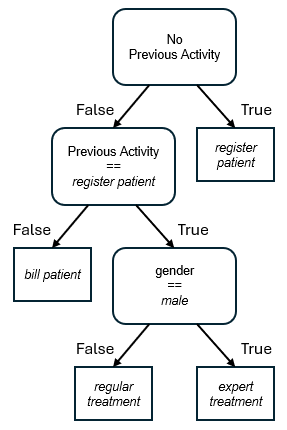
\includegraphics[width=0.4\textwidth]{gfx/decision_tree.png}
    \caption{
    A DT usable for next activity prediction in the process model shown in Figure \ref{fig:bpmn_example}.
    Leaf nodes are depicted as regular rectangles, while internal nodes are shown with rounded corners.
    Instead of raw feature indices and thresholds, the conditions used for splitting are expressed in natural language for better readability.
    The previous activity \textit{<PAD>} is a placeholder, if no previous activity has occured yet.
    }
    \label{fig:decision_tree}
\end{figure}

Since the structure of a DT explicitly represents the decision-making process,
it becomes immediately clear why they are widely regarded as white box models.
Each path from the root to a leaf corresponds to a set of human-readable decision rules,
enabling stakeholders to identify important features and assess the rationale behind each decision.

\subsection{Training Process}
\label{sec:dt_training}
Now that we understand how a DT makes predictions,
we turn our focus to the training process—how a DT is built from data.
Let $S$ be the collection containing the training data
and $|S|$ the amount of elements contained in $S$.
We assume the elements of $S$ to be tuples of the form $(x, y)$,
where $x = (x_1, ..., x_n)$ is a sample input and $y$ the corresponding target output label.
The training process aims to construct a structure that effectively partitions $S$ in a way,
such that the target labels $y$ within the partitions are as homogeneous as possible.
This is achieved by selecting the feature
and threshold for each split that maximize the "purity" of the resulting subsets.

A common metric used to evaluate this purity in data sets is \textbf{Gini impurity}.
The Gini impurity measures the likelihood of incorrectly classifying
a randomly chosen element, if it were labeled according to the distribution of labels.
Intuitively, it quantifies how "mixed" the labels are within $S$.
Mathematically, for $k$ different target labels,
where $p_i$ is the proportion of samples in $S$ having the $i$-th target label,
the Gini impurity is defined as:
\begin{align}
  G(S) = 1 - \sum_{i=0}^{k}p_i^2
\end{align}
The Gini impurity $G(S)$ ranges from $0$ to $1 - \frac{1}{k}$.
A value of $G(S) = 0$ indicates that $S$ is perfectly pure,
with all samples having a single target label,
while $G(S) = 1 - \frac{1}{k}$ represents a maximally impure dataset
where samples are evenly distributed among all $k$ target labels.
Generally, a lower $G(S)$ implies a higher purity.
\cite{decision_trees}

The training process begins at the root node,
which is associated with the entire training dataset $S$.
At each step, the algorithm evaluates all possible splits of the data by testing every feature $x_i$
and various thresholds.
Thresholds for splitting are derived directly from the values in the dataset associated with the node,
ensuring that every threshold capable of separating samples into distinct subsets is tested.
Specifically, given a feature $x_i$ and a sorted list of its values in the associated dataset,
potential thresholds are chosen as the midpoints between consecutive unique values.
Splits are chosen greedily, selecting the feature and threshold that provide the largest reduction in impurity.
Formally, if splitting $S$ into $S_1$ and $S_2$ results in Gini impurities $G(S_1)$ and $G(S_2)$,
the split is selected to minimize the weighted Gini impurity $G_{split}$:
\begin{align}
  G_{split}(S_1, S_2) = \frac{|S_1|}{|S|}G(S_1) + \frac{|S_2|}{|S|}G(S_2)
\end{align}
Once the best split is determined, two child nodes are created,
and each is associated with one of the datasets $S_1$ and $S_2$ resulting from the split.
This process is recursively repeated for each child node until a stopping criterion is met,
such as reaching a maximum tree depth, achieving a minimum number of samples per leaf,
or reducing impurity to a negligible level.

At the end of this recursive process,
the leaf nodes of the tree represent the terminal points of the decision-making structure.
Each leaf is associated with a subset of the training data
that corresponds to the sequence of splits leading to that leaf.
For our task of next activity prediction,
the output at each leaf is determined through majority voting:
the output label $y$ that occurs most frequently in the training samples
associated with the leaf is selected as the predicted label.


\subsection{Cost Complexity Pruning}
Depending on the selected stopping criterion,
the final DT may include subtrees with numerous nodes
that contribute little to the tree's predictive value.
This not only makes it more difficult to examine the tree's structures,
but may also hurt the overall accuracy of the DT due to overfitting.
To address this, pruning is a common technique used to simplify decision trees
by removing unnecessary branches, ultimately improving the tree's performance and interpretability.

One effective approach to pruning is \textbf{minimal cost-complexity pruning} \cite{decision_trees}.
This algorithm utilizes a complexity parameter $\alpha \ge 0$,
which balances the trade-off between a tree's complexity and its predictive performance.
Based on $\alpha$, the cost-complexity measure $C_{\alpha}$ of a given tree $T$ is defined as
\begin{align}
C_{\alpha}(T) = R(T) + \alpha |T|,
\end{align}
where $|T|$ is the number of leaf nodes in the tree, and $R(T)$ represents the total impurity of $T$,
computed as the total sample-weighted Gini impurity of the leaf nodes in $T$.
Minimal cost-complexity pruning finds the subtree $\bar{T}$ of $T$, such that the cost-complexity measure $C_{\alpha}(\bar{T})$ is minimized.
Since $\alpha$ penalizes tree complexity, larger values lead to more aggressive pruning.

The algorithm works by iteratively removing nodes from $T$.
Every iteration starts with computing the effective cost-complexity value $\alpha_t$ for each internal node $t$ as
\begin{align}
\alpha_t = \frac{R(t) - R(T_t)}{|T_t| - 1},
\end{align}
where $T_t$ is the subtree rooted at $t$.

The inner node $t$ with the smallest $\alpha_t$ is refered to as the weakest link in the tree.
If $\alpha_t \le \alpha$, this node and its subtree are pruned, meaning all its child nodes are removed, and it becomes a leaf node.
The pruning process continues iteratively until the minimal $\alpha_t$ in the remaining tree exceeds the predefined pruning parameter $\alpha$,
ensuring that the final tree retains only splits that contribute meaningfully to impurity reduction.

\section{Evaluation Metrics}
Having introduced both NNs and DTs,
we will go over the metrics we need to evaluate the performance of these models in our experiments.

\subsection{Accuracy}
Accuracy is a fundamental performance metric in machine learning
that measures the proportion of correctly predicted instances relative to the total number of instances.
For next activity prediction in PBPM,
accuracy evaluates how well the model correctly predicts the upcoming event in a process trace.
Given a set of predictions, the accuracy of the model is defined as:
\begin{align}
\text{Accuracy} = \frac{\text{\#(Correct predictions)}}{\text{\#(Total predictions)}}
\end{align}


\subsection{Demographic Parity}
While accuracy is a crucial metric for assessing overall model performance,
it does not account for potential biases in decision-making.
This necessitates the inclusion of fairness-aware quantitative measures
for assessing and comparing models to ensure that they meet fairness criteria
alongside performance metrics.

One possible perspective on discrimination is provided by \textbf{group fairness} metrics,
which offer a way to assess whether a machine learning model's predictions are equitable across different groups within the population.
In PBPM, these metrics help ensure that predictions, such as the next activity or outcome in a business process,
do not favor one group over another based on sensitive attributes.
These \textbf{sensitive attributes} refer to characteristics of individuals or groups
that are typically protected by laws or ethical guidelines due to their potential to lead to biased or discriminatory treatment,
such as gender, ethnicity, age, disability status, etc.

In this thesis, we utilize on one of the most prevalent fairness metrics, \textbf{demographic parity} \cite{demographic_parity},
which quantifies the disparity in positive prediction rates across different demographic groups. 
Let $y$ be the prediction of the model, that is either categorized as positive for $y = 1$ or negative for $y = 0$.
Moreover let $S$ be a sensitive attribute whose values can be split into the demographic groups $s_1$ and $s_2$.
A model satisfies demographic parity if the probability of receiving a positive prediction $y = 1$
is independent of the sensitive attribute $S$, meaning:
\begin{align}
P(y = 1 \mid S = s_1) = P(y = 1 \mid S = s_2)
\end{align}
Based on the definition of demographic parity, the discrimination can be measured as the difference in selection rates,
commonly referred to as $\Delta \textit{DP}$, similar to how it is defined in \cite{fairness_foundation}:
\begin{align}
%\Delta \textit{DP} = \left\vert \frac{\#(\text{Samples} \mid y = 1, S = s_1)}{\#(\text{Samples} \mid S = s_1)} - \frac{\#(\text{Samples} \mid y = 1, S = s_2)}{\#(\text{Samples} \mid S = s_2)} \right\vert
\Delta \textit{DP} = \left\vert P(y = 1 \mid S = s_1) - P(y = 1 \mid S = s_2) \right\vert
\end{align}
Since the true probabilities are unknown, they are estimated from the model's predictions for available samples,
using the observed selection rates for each demographic group as:
\begin{align}
P(y = 1 \mid S = s_i) \approx \frac{\#(\text{Samples} \mid y = 1, S = s_i)}{\#(\text{Samples} \mid S = s_i)}, i \in \{1,2\}
\end{align}
$\Delta \textit{DP}$ ranges between the values 0 and 1.
A smaller $\Delta \textit{DP}$ indicates that the model's predictions are more equitable across demographic groups,
whereas a larger $\Delta \textit{DP}$ suggests a potential bias in the model's decision-making process.

As an example, let's consider the process model shown in Figure \ref{fig:bpmn_example},
where a gateway after the \textit{register patient} activity determines whether a patient
is assigned to an \textit{expert examination} or a \textit{regular examination}.
To evaluate whether a machine learning model makes fair predictions at this decision point,
we can use samples where the previous activity was \textit{register patient}.
These samples are split into demographic groups based on \textit{gender}, distinguishing between \textit{male} and \textit{female} patients.
In this context, the positive prediction is defined as the assignment to \textit{expert examination}, while any other outcome is considered negative.

Suppose the model assigns 70\% of male patients to \textit{expert examination} and 30\% of female patients to \textit{expert examination},
as is done in the underlying process model.
The $\Delta \textit{DP}$ is then computed as
$\Delta \textit{DP} =
\vert P(y = \textit{expert examination} \mid \textit{gender} = \textit{male}) - P(y = \textit{expert examination} \mid \textit{gender} = \textit{female}) \vert =
\vert 0.7 - 0.3 \vert = 0.4$.

This result reflects the disparity in selection rates, indicating that the model disproportionately assigns one of the demographic groups to expert examinations.
By measuring and minimizing $\Delta \textit{DP}$,
we aim to ensure that predictive models used in PBPM do not systematically favor one demographic group over another,
thus improving fairness in the decision-making processes.


\section{Formalized Problem Statement}
Having cleared all the preliminaries, we can now present a formalized problem statement.
Given a classifier $C_{\text{enriched}}$ for next activity prediction, which has access to all sensitive attributes,
its predictions may inadvertently exhibit unfairness for certain decisions and demographic groups,
as measured by demographic parity disparity ($\Delta \textit{DP}$).
The objective of this thesis is to mitigate such unfairness while maintaining high predictive performance.

To address this issue, we aim to derive a modified classifier $C_{\text{modified}}$
that reduces the observed $\Delta \textit{DP}$ in $C_{\text{enriched}}$, thereby enhancing fairness in decision-making.
However, this fairness enhancement should not come at the cost of excessive performance degradation.
Therefore, $C_{\text{modified}}$ must achieve an accuracy greater than that of a baseline classifier $C_{\text{base}}$,
which does not utilize any sensitive attributes and is, by design, demographically fair.

The reduction of unfair demographic disparities is guided by domain-specific considerations,
ensuring that only those disparities deemed unfair within the context of the process are addressed.
This is achieved through a knowledge distillation approach, which enables a domain expert to analyze and refine the decision-making process of the model.
The precise details of this methodology are outlined in the next chapter.